\section{Results}
All timings below are the arithmetic mean of three repetitions, obtained on the 8-core workstation described in Section~6. The complete raw dataset is available in \texttt{results\_raw.csv}, and the aggregated per-configuration values (including speedup and efficiency) in \texttt{results.csv}. The sequential baselines were $T_{seq} = 0.68$~s, $2.59$~s and $10.26$~s for $N = 500$, $1000$ and $2000$ respectively.

\subsection{Execution time}
Table~\ref{tab:exectime} reports the total execution time of the 2D implementation as a function of the number of processes $p$ and the grid size $N$; Figure~\ref{fig:exectime} plots the same data on a logarithmic scale. The runtime decreases sharply up to $p = 4$, after which it \emph{increases} again at $p = 8$. Since the machine has only 8 physical cores, at $p = 8$ every core hosts one MPI process and the operating system, the timing barriers, and the memory subsystem all compete for the same resources; the communication cost (see Section~7.4) then outweighs the shrinking computational work.

\begin{table}[h]
\centering
\caption{Mean total execution time [s], 2D decomposition.}
\label{tab:exectime}
\begin{tabular}{lcccc}
\toprule
$N$ & $p=1$ & $p=2$ & $p=4$ & $p=8$ \\
\midrule
500  & 0.639 & 0.357 & 0.350 & 0.475 \\
1000 & 2.381 & 1.256 & 0.800 & 1.285 \\
2000 & 9.238 & 4.724 & 2.752 & 3.875 \\
\bottomrule
\end{tabular}
\end{table}

\begin{figure}[h]
\centering
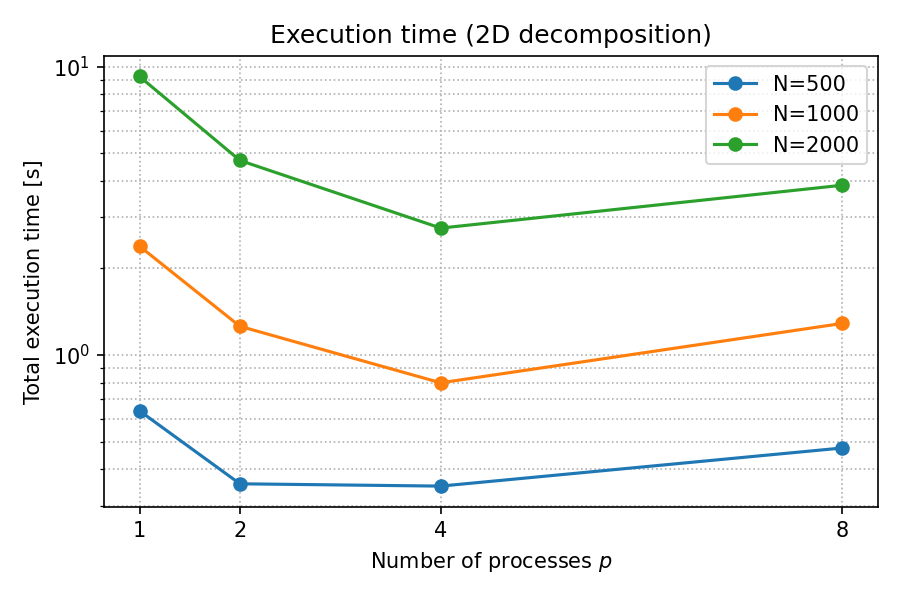
\includegraphics[width=0.62\textwidth]{figures/exec_time.png}
\caption{Total execution time versus the number of processes (2D, log scale).}
\label{fig:exectime}
\end{figure}

\subsection{Speedup and efficiency}
The speedup is defined as $S(p) = T_{base}/T(p)$ and the efficiency as $E(p) = S(p)/p$, using the sequential baseline $T_{base}$ for each grid size. Table~\ref{tab:speedup} and Figures~\ref{fig:speedup}--\ref{fig:efficiency} summarise the results for the 2D decomposition.

The best speedup is obtained at $p = 4$ and grows with the problem size: from $1.96\times$ at $N = 500$ to $3.73\times$ at $N = 2000$. This is the expected behaviour of a memory-bound stencil computation: larger grids increase the computation-to-communication ratio, so the fixed halo-exchange overhead is better amortised (the surface-to-volume effect). Efficiency stays close to $0.9$--$1.0$ up to $p = 2$, remains high ($\approx 0.93$) at $p = 4$ for the largest grid, but collapses at $p = 8$ because of core oversubscription and communication overhead.

\begin{table}[h]
\centering
\caption{Speedup $S(p)$ and efficiency $E(p)$, 2D decomposition.}
\label{tab:speedup}
\begin{tabular}{lcccccc}
\toprule
 & \multicolumn{2}{c}{$N=500$} & \multicolumn{2}{c}{$N=1000$} & \multicolumn{2}{c}{$N=2000$} \\
\cmidrule(lr){2-3}\cmidrule(lr){4-5}\cmidrule(lr){6-7}
$p$ & $S$ & $E$ & $S$ & $E$ & $S$ & $E$ \\
\midrule
1 & 1.07 & 1.07 & 1.09 & 1.09 & 1.11 & 1.11 \\
2 & 1.92 & 0.96 & 2.06 & 1.03 & 2.17 & 1.09 \\
4 & 1.96 & 0.49 & 3.24 & 0.81 & 3.73 & 0.93 \\
8 & 1.44 & 0.18 & 2.01 & 0.25 & 2.65 & 0.33 \\
\bottomrule
\end{tabular}
\end{table}

\begin{figure}[h]
\centering
\begin{minipage}{0.49\textwidth}
\centering
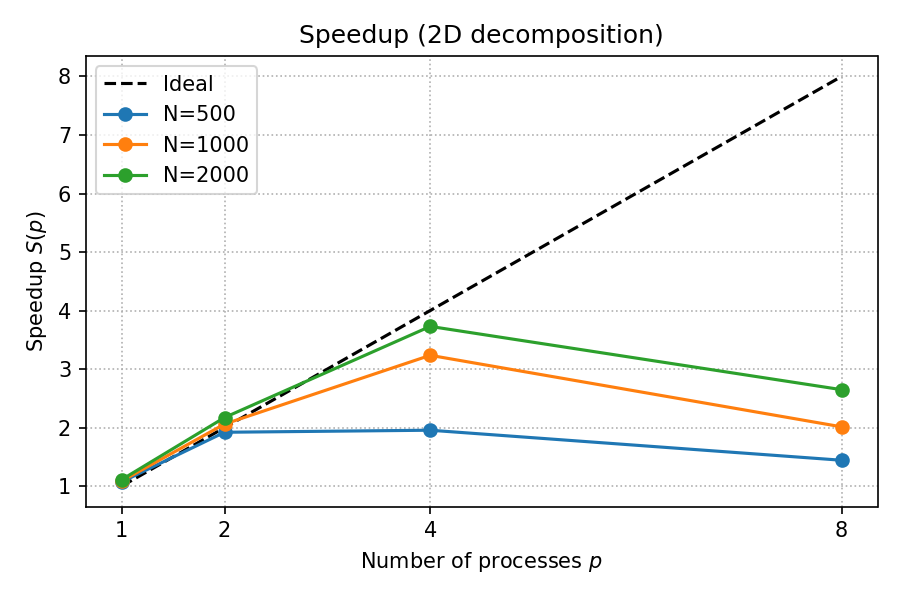
\includegraphics[width=\textwidth]{figures/speedup.png}
\caption{Speedup $S(p)$ (2D).}
\label{fig:speedup}
\end{minipage}\hfill
\begin{minipage}{0.49\textwidth}
\centering
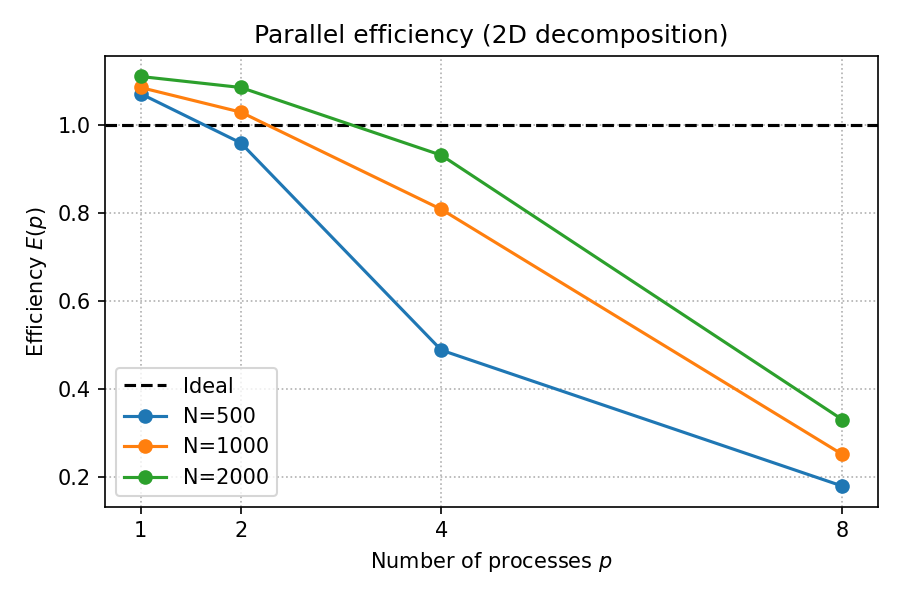
\includegraphics[width=\textwidth]{figures/efficiency.png}
\caption{Efficiency $E(p)$ (2D).}
\label{fig:efficiency}
\end{minipage}
\end{figure}

The super-unitary efficiency observed at $p = 1$--$2$ ($E > 1$) is a mild super-linear artifact: the MPI implementation reuses pre-allocated ghost buffers, whereas the sequential baseline re-pads the whole array with \texttt{np.pad} at every step, and the smaller per-process working set fits better in cache.

\subsection{Comparison across topologies}
Table~\ref{tab:topology} contrasts the 1D (row-slab) and 2D (block) decompositions at $N = 2000$; Figure~\ref{fig:topology} plots the two curves. Contrary to the asymptotic argument of Section~4---where the 2D scheme exchanges $\mathcal{O}(N/\sqrt{p})$ elements against $\mathcal{O}(N)$ for the 1D scheme---the two topologies perform almost identically up to $p = 4$, and the 1D layout is actually \emph{faster} at $p = 8$ ($3.39$~s vs.\ $3.88$~s).

The explanation is that, at these small process counts on a shared-memory node, the halo cost is dominated by \emph{message count and latency} rather than by message \emph{volume}. The 1D decomposition issues only two \texttt{Sendrecv} calls per step (North/South) against up to four for the 2D block, and the shared-memory bandwidth makes the larger 1D messages essentially free. The theoretical advantage of the 2D volume scaling would only emerge at much larger $p$ on a real distributed-memory interconnect.

\begin{table}[h]
\centering
\caption{Total execution time [s]: 1D vs.\ 2D at $N=2000$.}
\label{tab:topology}
\begin{tabular}{lcccc}
\toprule
Decomp. & $p=1$ & $p=2$ & $p=4$ & $p=8$ \\
\midrule
1D & 9.223 & 4.683 & 2.680 & 3.388 \\
2D & 9.238 & 4.724 & 2.752 & 3.875 \\
\bottomrule
\end{tabular}
\end{table}

\begin{figure}[h]
\centering
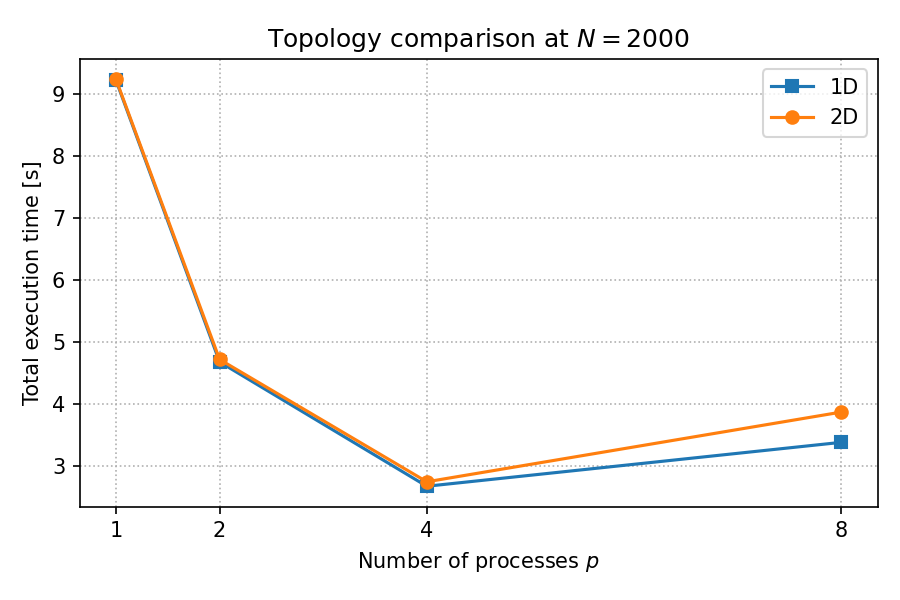
\includegraphics[width=0.6\textwidth]{figures/topology.png}
\caption{1D vs.\ 2D total execution time at $N=2000$.}
\label{fig:topology}
\end{figure}

\subsection{Computation vs. communication}
Figure~\ref{fig:commcompute} shows the per-process time split between the halo-exchange and the grid computation for $N = 2000$ (2D). The computation time halves with every doubling of $p$ (from $9.23$~s at $p=1$ down to $1.83$~s at $p=8$), confirming that the computational phase scales almost ideally. The communication time, on the contrary, grows steadily and becomes the dominant term at $p = 8$, where it accounts for roughly $53\%$ of the total runtime ($2.04$~s of comm against $1.83$~s of compute). This crossover is precisely what caps the achievable speedup on this machine.

\begin{table}[h]
\centering
\caption{Mean per-process computation/communication split ($N=2000$, 2D).}
\label{tab:commcompute}
\begin{tabular}{lcccc}
\toprule
 & $p=1$ & $p=2$ & $p=4$ & $p=8$ \\
\midrule
Computation [s] & 9.232 & 4.664 & 2.595 & 1.833 \\
Communication [s] & 0.006 & 0.056 & 0.153 & 2.037 \\
Comm.\ fraction & 0.1\% & 1.2\% & 5.6\% & 52.6\% \\
\bottomrule
\end{tabular}
\end{table}

\begin{figure}[h]
\centering
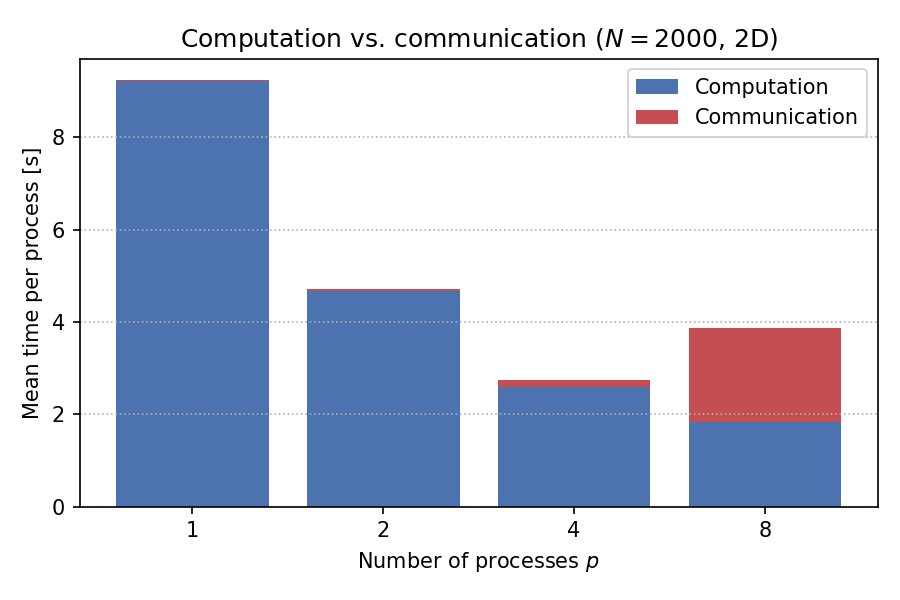
\includegraphics[width=0.6\textwidth]{figures/comm_compute.png}
\caption{Stacked computation vs.\ communication time per process ($N=2000$, 2D).}
\label{fig:commcompute}
\end{figure}

\subsection{Scalability}
Finally, we assess weak scaling by keeping the workload per process fixed at approximately $500 \times 500$ cells and increasing both the grid size and the process count together ($N = 500\sqrt{p}$). Ideal weak scaling would keep the total runtime constant. Figure~\ref{fig:weak} shows that the \emph{computation} time is indeed almost flat (it stays in the $0.64$--$0.85$~s band across $p = 1 \to 16$), which validates the load balancing of the decomposition. The \emph{total} runtime, however, drifts upward: it doubles from $p=1$ ($0.64$~s) to $p=4$ ($0.80$~s, weak efficiency $0.80$), and then degrades sharply for $p = 9$ and $p = 16$. The latter two points require \emph{oversubscribing} the 8 physical cores, so their inflation is a hardware artifact rather than an algorithmic one, and it is again driven by the communication term.

\begin{table}[h]
\centering
\caption{Weak scaling (2D, $\approx 500\times500$ cells/process). Points $p=9,16$ oversubscribe the 8 cores.}
\label{tab:weak}
\begin{tabular}{lcccc}
\toprule
$p$ (grid $N$) & 1 (500) & 4 (1000) & 9 (1500) & 16 (2000) \\
\midrule
Total time [s]   & 0.639 & 0.800 & 1.660 & 3.481 \\
Compute time [s] & 0.636 & 0.640 & 0.793 & 0.849 \\
Weak efficiency  & 1.00 & 0.80 & 0.39 & 0.18 \\
\bottomrule
\end{tabular}
\end{table}

\begin{figure}[h]
\centering
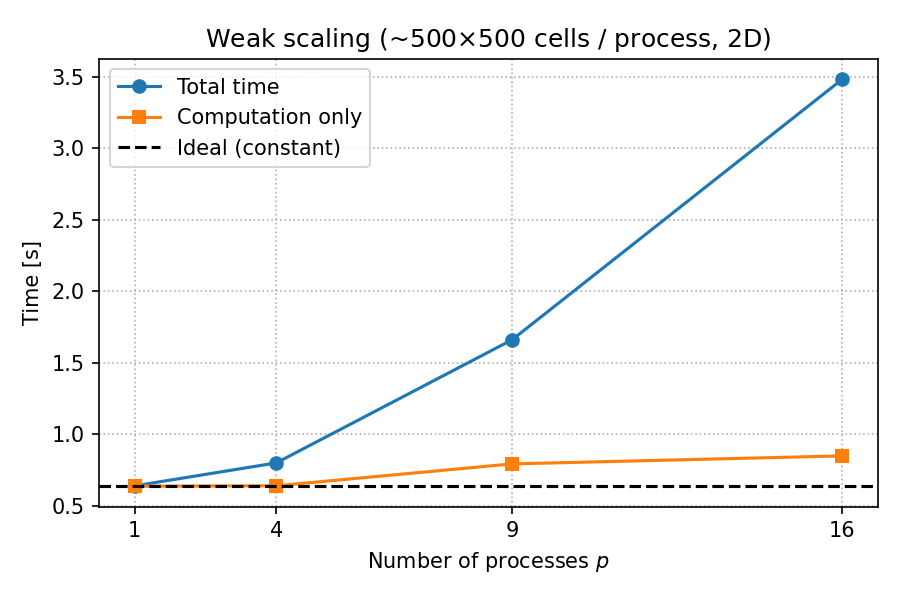
\includegraphics[width=0.6\textwidth]{figures/weak_scaling.png}
\caption{Weak scaling: total and computation-only time per process.}
\label{fig:weak}
\end{figure}
